% !TeX spellcheck = en_US
\documentclass[11pt,a4paper,sans]{moderncv}

%% Character encoding
\usepackage[utf8]{inputenc}
\usepackage{graphicx}

%% ModernCV themes
\moderncvstyle{classic}
\moderncvcolor{black}
%\renewcommand{\familydefault}{\sfdefault}
\nopagenumbers{}

% Japanese
\usepackage{CJKutf8}

% Russian
%\usepackage[russian]{babel}

%% Adjust the page margins
\usepackage[margin=1.8cm]{geometry}
\setlength{\hintscolumnwidth}{3.5cm}

\newcommand{\mycvitemwithcomment}[3]{\cvitemwithcomment{\parbox{0.2\textwidth}{\vspace{-\baselineskip}\flushright #1}}{\parbox{10cm}{#2}}{#3}\vspace{0.5\baselineskip}}

%% Personal data
\firstname{Maciej P.}
\familyname{Kopeć}
\address{Na Popielówkę 75P/2}{32-087 Zielonki, Poland}
\mobile{+48 515 083 938}
\email{maciej.p.kopec@gmail.com}
\extrainfo{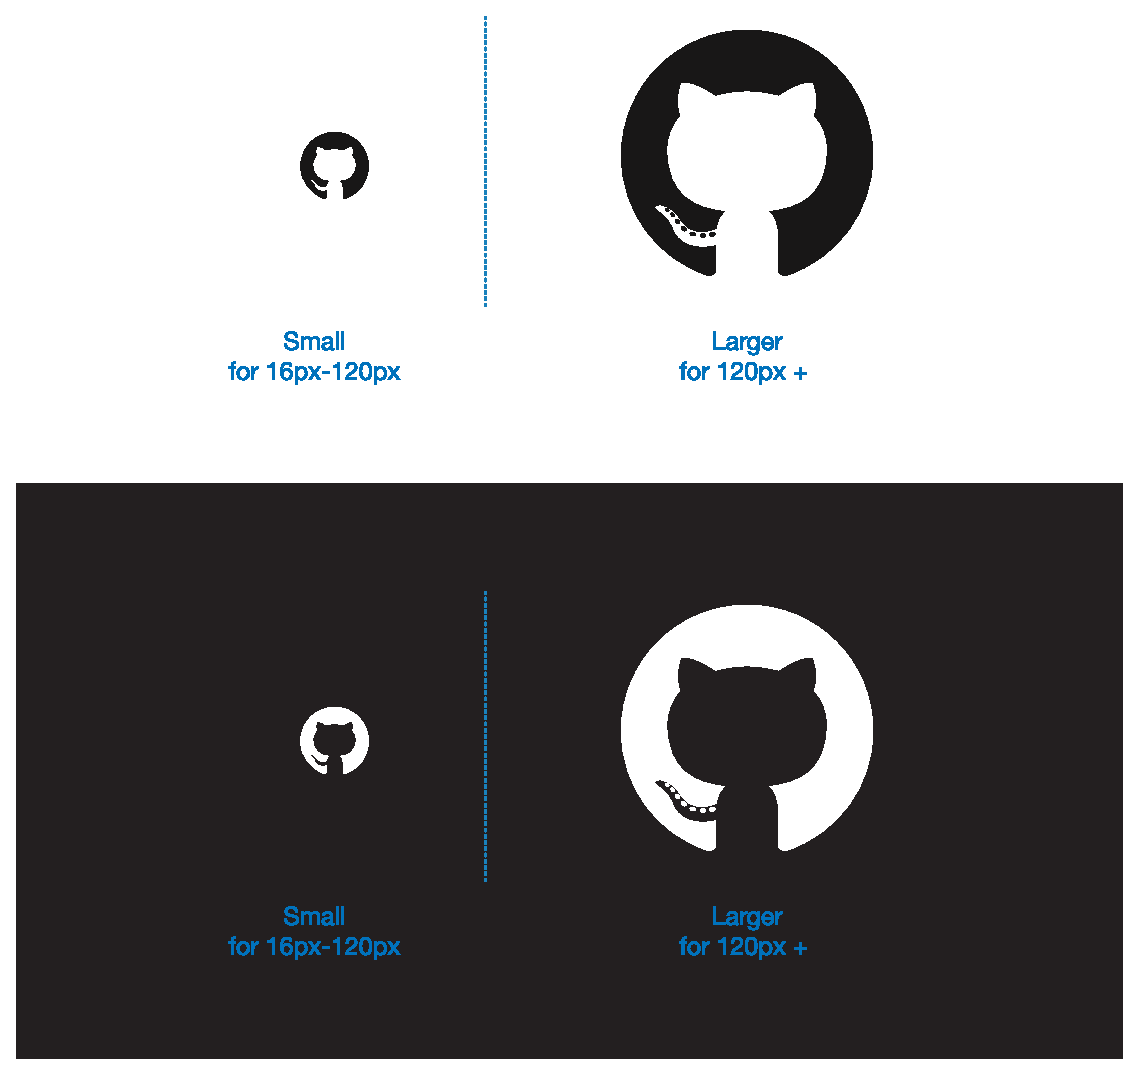
\includegraphics[height=1em, trim={4.8cm 14.55cm 12.76cm 1.95cm}, clip]
	{img/GitHub-Mark.eps}
GitHub: \href{https://github.com/mpkopec}{mpkopec}}
%\photo[80pt][0.4pt]{mkopec.jpg}

%%------------------------------------------------------------------------------
%% Content
%%------------------------------------------------------------------------------
\begin{document}
\makecvtitle

\section{Education}
\cventry{2014--2015}{MSc}{\textbf{AGH-UST}}{\textbf{Cracow}}{5.0}{Major: \textbf{Technical Physics} at~Faculty of~Physics and~Applied Computer Science}
\cventry{2010--2014}{BSc}{\textbf{AGH-UST}}{\textbf{Cracow}}{\textit{4.5}}{Major: \textbf{Technical Physics} at~Faculty of~Physics and~Applied Computer Science}

\section{Professional experience}
\cventry{April 2019 -- present}{Electronics Engineer}{Merit Poland sp. z 
o.o}{}{}{}
\cvitem{}{At Merit, my current responsibilities include: designing electronic circuits for automotive purposes;
electrical simulations and data analysis (including scripting); component database maintenance
and development; ECAD tools integration process; tests and measurements of the designed circuits
and supporting and mentoring interns.}

\cventry{January 2018 -- March 2019}{Electronics Engineer}{Sii Poland}{}{}{}
\vspace{-\baselineskip}
\cvitem{}{At Sii I was delegated to work as a contractor in Merit Poland sp.~z~o.o. There I was
	responsible for designing electronic circuits for automotive purposes;
	electrical simulations and data analysis (including scripting); component database maintenance
	and development; ECAD tools integration process; tests and measurements of the designed circuits;
	supporting and mentoring interns.}

\cventry{December 2014 -- December 2017}{Beam diagnostics and Instrumentation Specialist}{National
	Synchrotron Radiation Centre `Solaris'}{}{}{}
\cvitem{}{At NSRC `Solaris' my tasks were: designing electronic readout and measurement
systems; electronic prototyping and reworks; beam instrumentation design, assembly, maintenance
(including scripting, setup, etc.) and diagnostics; beam diagnostic data analysis; electronic 
simulations and data analysis.}

\cventry{May 2016 -- \linebreak August 2016}{Embedded systems developer}{Organisation Européenne
	 pour la Recherche Nucléaire (CERN)}{}{}{}
\cvitem{}{At CERN I was tasked with: development of 1G ethernet link on ZC706 evaluation board;
detector readout systems testing and debugging and setting up development environments for
detector readout systems.}

\cventry{January 2014 -- \linebreak June 2014}{Hardware development intern}{Woodward Poland sp. z o.o.}{}{}{}
\vspace{-\baselineskip}
\cvitem{}{As an intern at Woodward Poland, I was working on: electrical circuit design (including
	PCB design); testing and preparing prototypes; measurements and data analysis, as well as
RoHS directive compliance verification.}

\cventry{July 2013 -- \linebreak August 2013}{Electrical engineering trainee}{Faculty of~Physics
	and~Applied Computer Science}{}{}{}
\vspace{-\baselineskip}
\cvitem{}{Programming microcontrollers with ARM Cortex-M3 core.}

\cventry{2008--2013}{Web-developer}{Back-end and front-end web development}{}{}{}
\cvitem{}{As a web developer I was working on: HTML, CSS and jQuery front-end design; preparing
custom Wordpress templates; writing plugins and snippets for Joomla! and Wordpress systems
and developing independent back-end applications in PHP and MySQL.}


\section{Courses and certificates}

%\mycvitemwithcomment{In progress}{Advanced PCB Layout Course}{FEDEVEL~Academy}
%\vspace{-.5\baselineskip}
\mycvitemwithcomment{November 2018}{EMC for automotive \hspace{-7.5cm}}{EMC 
Solution}
\vspace{-.5\baselineskip}
\mycvitemwithcomment{October 2017}{Advanced Hardware Design 
\hspace{-7.5cm}}{FEDEVEL~Academy}
\vspace{-.5\baselineskip}
\mycvitemwithcomment{June 2017}{Accelerator Power Electronics 
Engineering (Grade: Excellent)}{USPAS June 2017}
\vspace{-.5\baselineskip}
\mycvitemwithcomment{June 2017}{Pulsed Power Engineering (Grade: 
Outstanding)}{USPAS June 2017}
\vspace{-.5\baselineskip}
\mycvitemwithcomment{December 2016}{Learn Altium Essentials}{FEDEVEL~Academy}
\vspace{-.5\baselineskip}
\mycvitemwithcomment{April 2016}{PCB design at RF --- multi-Gigabit 
transmission, EMI control and PCB materials}{Cadence GmbH}
\vspace{-.5\baselineskip}
\mycvitemwithcomment{April 2016}{Essential high-speed PCB design for signal integrity}{Cadence GmbH}
\vspace{-.5\baselineskip}

\section{Recent publications}
\cvlistitem{M.P. Kopeć et~al., \emph{Universal digital aggregator for in-line 
signal processing}, 
IPAC~2017}

\cvlistitem{A.I. Wawrzyniak et~al., \emph{Performance of Solaris storage 
ring}, IPAC 2017}
\cvlistitem{ A. Kisiel et~al., \emph{Beta function measurement in the Solaris 
storage ring}, IPAC 2017}

\section{University and private projects}
\cventry{July 2014 -- \\Sptember 2015}{Master thesis}{}{}{}{{\large Subject: Control interface for SALT ASIC for LHCb detector tracker upgrade}}
\cvitem{}{Hardware I\textsuperscript{2}C interface implementation in Verilog.}

\cventry{July 2013 -- \\ October 2013}{Bachelor thesis}{}{}{}{{\large Subject: Demo application for colour touchscreen working in embedded system}}
\cvitem{}{Design and~implementation of~GUI library for~LPC1768 microcotroller 
with a~demo application.}

\section{Other skills}

\cvitemwithcomment{\parbox{0.2\textwidth}{\vspace{-\baselineskip}\flushright 
Programming languages}}{\parbox{13cm}{C, C++ (basic), Python, Verilog, 
SystemVerilog, LabView (basic), VHDL, SQL (more than basic), MATLAB (basic), 
Simulink(basic)}}{}
\vspace{0.5\baselineskip}
\cvitemwithcomment{Design software}{\parbox{13cm}{KiCad, Altium Designer,
Mentor Xpedition, LTspice IV, Xilinx Vivado (more than basic), Xilinx Vitis (basic),
Eclipse}}{}
\vspace{0.5\baselineskip}
\cvitemwithcomment{\parbox{0.2\textwidth}{\vspace{-\baselineskip}\flushright 
Other software and~technologies}}{\parbox{13cm}{Linux, \LaTeX, git, Wordpress, 
MS Office, Vim}}{}
\vspace{0.5\baselineskip}
\cvitemwithcomment{\parbox{0.2\textwidth}{\vspace{-\baselineskip}\flushright 
Additional qualifications}}{\parbox{13cm}{SEP 1\hspace{3pt}kV~license 
(30\hspace{3pt}kV for laboratory testing), driving 
license, good knowledge of~circuits and~signals theory, coping with 
analytical problems}}{}

\section{Languages}

\cvitemwithcomment{English}{Fluent (FCE passed in 2007)}{}
\cvitemwithcomment{Russian}{Basic}{}
\cvitemwithcomment{Japanese}{Semi-intermediate}{Learning in progress}

\section{Interests}
\cvitem{}{volleyball, cycling, books, DIY, snooker, e-sports, physics.}

\section{Disclaimer}

I agree to the processing of personal data provided in this document for 
realising the recruitment process pursuant to the Personal Data Protection Act 
of 10 May 2018 (Journal of Laws 2018, item 1000) and in agreement with 
Regulation (EU) 2016/679 of the European Parliament and of the Council of 27 
April 2016 on the protection of natural persons with regard to the processing 
of personal data and on the free movement of such data, and repealing Directive 
95/46/EC (General Data Protection Regulation).


\bibliography{publications}
\end{document}